\begin{frame}
\frametitle{Applications}
Deux applications développées
\begin{description}
	\item [Graphique] développement de programmes
	\item [CLI] calculs intensifs
\end{description}
\end{frame}

\subsection{Application graphique}

\begin{frame}
\frametitle{Application graphique v0.1}
\begin{center}
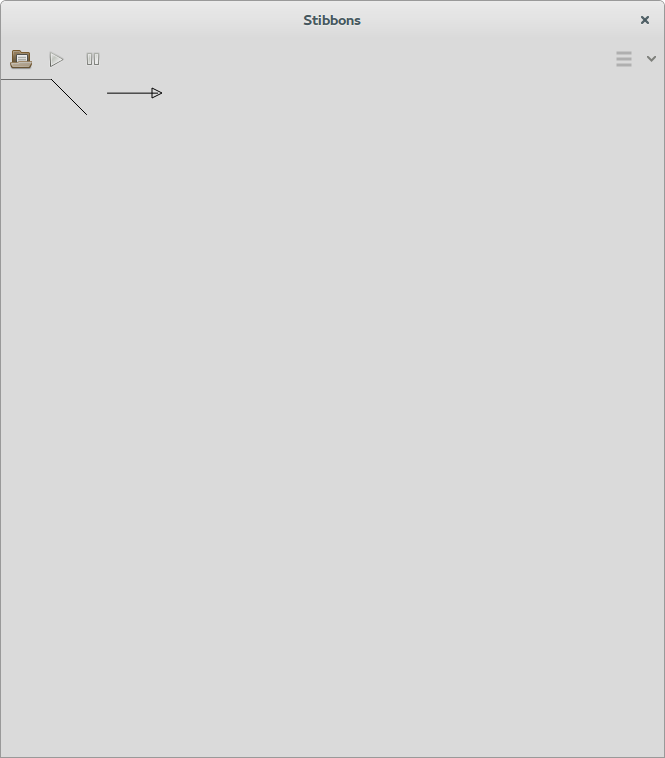
\includegraphics[scale=0.16]{doc/Presentation/screenshot/stibbons-0-1-2.png}
\end{center}

\begin{itemize}
	\item Origine dans le coin supérieur gauche
	\item Une tortue par défaut
	\item Tortue = triangle noir creux
	\item Les tortues peuvent tracer des lignes
	\item Impossible d'ouvrir plusieurs programmes
\end{itemize}
\end{frame}

\begin{frame}
\frametitle{Application graphique v0.2}
\begin{center}
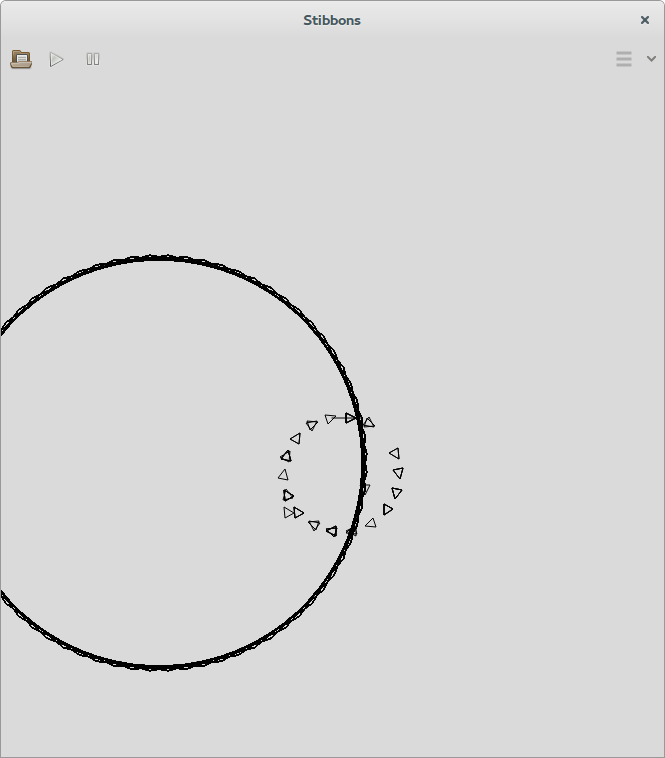
\includegraphics[scale=0.16]{doc/Presentation/screenshot/stibbons-0-2-2.png}
\end{center}

\begin{itemize}
	\item Origine centrée
\end{itemize}
\end{frame}

\begin{frame}
\frametitle{Application graphique v0.3}
\begin{center}
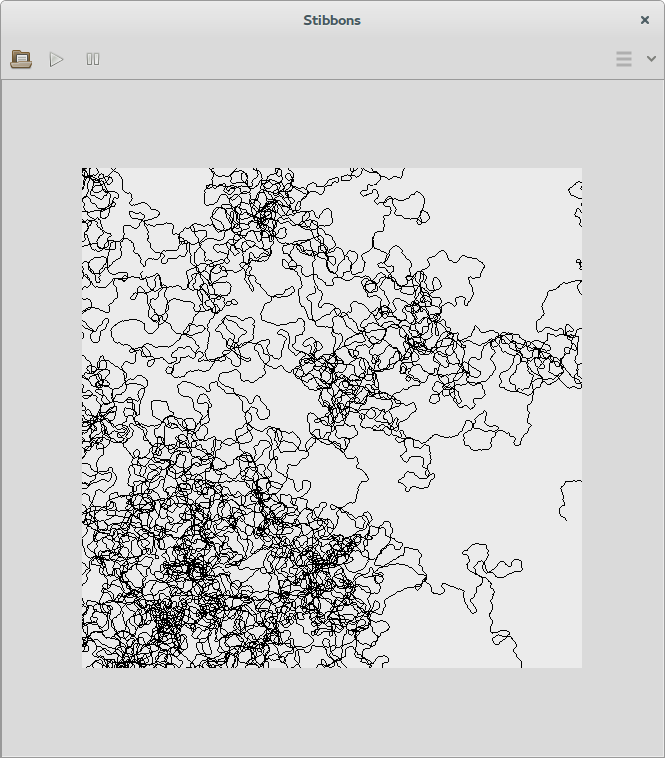
\includegraphics[scale=0.16]{doc/Presentation/screenshot/stibbons-0-3-2.png}
~~~~~~~~
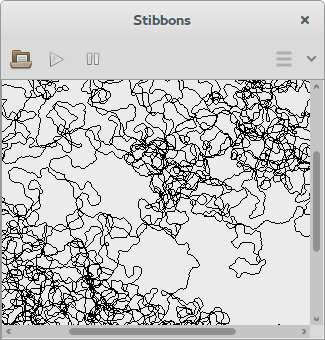
\includegraphics[scale=0.16]{doc/Presentation/screenshot/stibbons-0-3-3.png}
\end{center}

\begin{itemize}
	\item Monde borné, centré
	\item Tortues colorées, dessinées pleines
	\item Lignes colorées
	\item Zones visibles et colorées
	\item Performances de dessin améliorées
\end{itemize}
\end{frame}

\begin{frame}
\frametitle{Application graphique v0.4}
\begin{center}
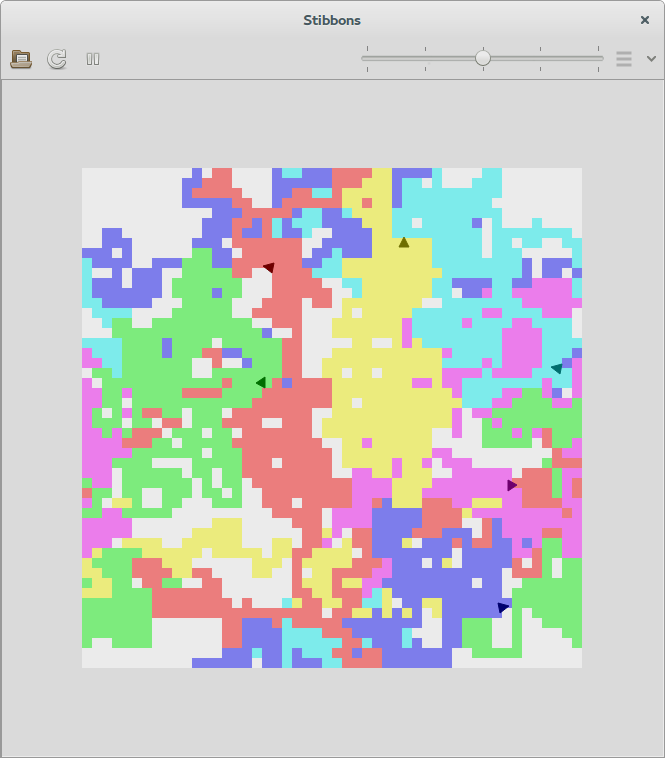
\includegraphics[scale=0.16]{doc/Presentation/screenshot/stibbons-0-4-2.png}
\end{center}

\begin{itemize}
	\item Gestion de la vitesse
	\item Démarrage, pause et redémarrage
	\item Export du modèle
	\item Ouverture de plusieurs fichiers
	\item Bords rebouclants en option
	\item Plus de tortue par défaut
\end{itemize}
\end{frame}

\begin{frame}
\frametitle{Application graphique v1.0}
\begin{center}
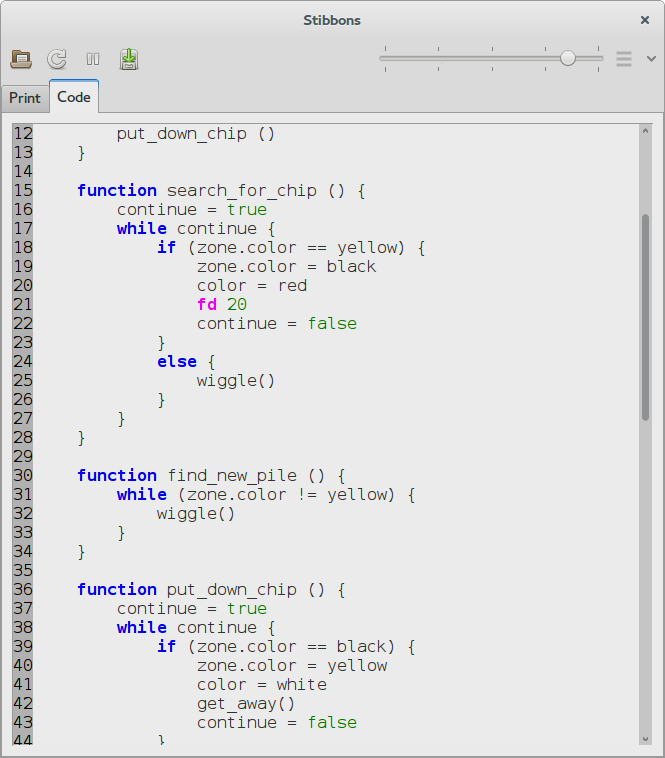
\includegraphics[scale=0.16]{doc/Presentation/screenshot/stibbons-0-5-2.png}
~~~~~~~~
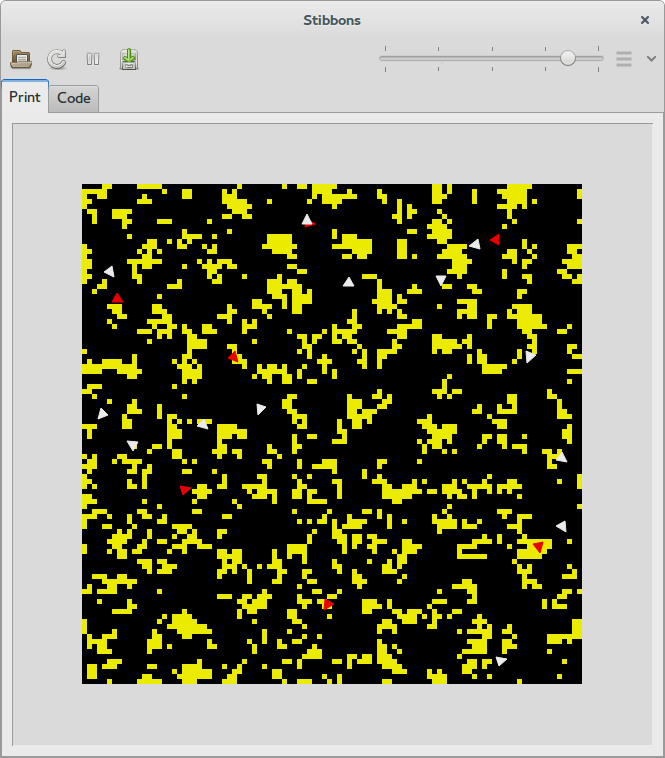
\includegraphics[scale=0.16]{doc/Presentation/screenshot/stibbons-0-5-3.png}
\end{center}

\begin{itemize}
	\item Editeur de texte
	\item Ajout de raccourcis clavier
	\item Bords rebondissants en option
\end{itemize}
\end{frame}

\begin{frame}
\frametitle{Application graphique v1.1}
\begin{center}
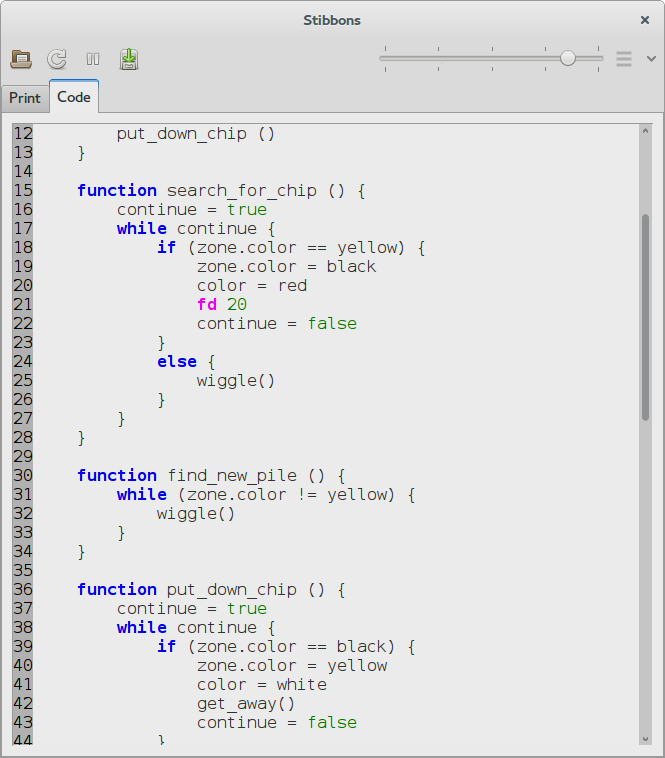
\includegraphics[scale=0.16]{doc/Presentation/screenshot/stibbons-0-5-2.png}
~~~~~~~~
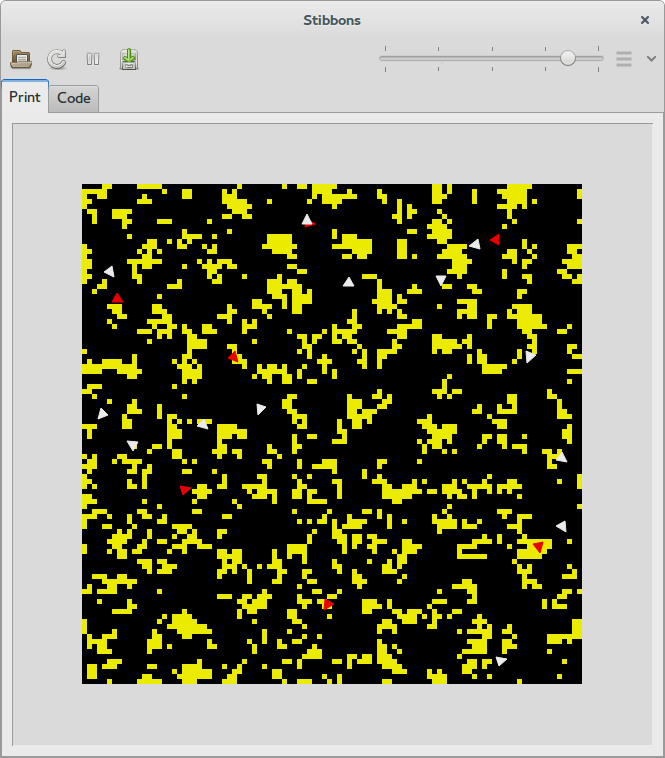
\includegraphics[scale=0.16]{doc/Presentation/screenshot/stibbons-0-5-3.png}
\end{center}

\begin{itemize}
	\item Corrections de grave fuite mémoire
	\item Correction d'erreur sémantique inexacte
	\item Amélioration de la coloration syntaxique
\end{itemize}
\end{frame}

\subsection{Application CLI}

\begin{frame}
\frametitle{Application CLI}

Utilisation~: stibbons-cli [options] fichier

Options~:
\begin{description}
	\item[\texttt{-{}-}export s] Exporte le modèle toutes les \emph{s} secondes
	\item[\texttt{-{}-}prefix p] Préfixe les fichiers exportés avec \emph{p}
	\item[\texttt{-{}-}png] Génère une image PNG pour chaque export
	\item[\texttt{-{}-}no-json] N'exporte pas le modèle dans un fichier JSON
\end{description}

Arguments~:
\begin{description}
	\item[fichier] Le fichier de programme Stibbons à exécuter
\end{description}

\end{frame}

